\documentclass[journal,onecolumn]{IEEEtran}

\usepackage{graphicx} % Required for inserting images
\usepackage{geometry}
\usepackage{minted}
\usepackage{hyperref}
\usepackage{mathtools}
\usepackage{enumitem}
\usepackage{amssymb}
\usepackage{float}

\DeclareMathOperator{\dom}{dom}
\geometry{letterpaper, margin = 1in}

\def\BibTeX{{\rm B\kern-.05em{\sc i\kern-.025em b}\kern-.08em
    T\kern-.1667em\lower.7ex\hbox{E}\kern-.125emX}}


\begin{document}
\title{
Subgradient Methods Applied to LASSO Regression
}

\author{\IEEEauthorblockN{Kasey Tian}
\IEEEauthorblockA{\textit{Electrical and Computer Engineering} \\
\textit{Rutgers University}\\
New Brunswick, NJ, USA \\
kasey.tian@rutgers.edu}
}


\maketitle

\begin{abstract}
Subgradient methods
\end{abstract}

\begin{IEEEkeywords}
optimization, subgradients, LASSO, regression
\end{IEEEkeywords}

\section{Introduction}\label{sec:intro}
Subgradient methods are a way to perform an optimization on an objective function which is not fully differentiable. For non-differentiable objective functions, traditional methods, such as gradient descent and Newton's method, are impossible to execute. They can also be combined with a wide variety of other optimization methods, and have far reaching applications. They were originally developed by Shor and others in the Soviet Union in the 1960s and 70s \cite{boydparksubgradients} \cite{boydxiaosubgradients}. LASSO regression is a regression analysis method which was first introduced in 1986 \cite{lassooriginal} in the field of geophysics, but was then independently rediscovered, named, and popularized in 1996 by Tibshirani \cite{lassopaper}. It is characterized by regularization using the \(L_1\) norm, which involves the absolute value function and is therefore not fully differentiable. This makes it a prime candidate for applying subgradient methods. To demonstrate a practical implementation LASSO regression will be used with a linear classifier to predict life expectancy from World Health Organization (WHO) data.


\section{Mathematical Analysis}\label{sec:math}
In this section we will explore the mathematics of subgradients, subgradient methods and LASSO regression.
\subsection{Defining Subgradient}\label{sec:math subgrad}
This section is mostly adapted from \cite{boydvandenberghesubgradient}, with some supplementary material from \cite{boydparksubgradients}.
\subsubsection{Definitions}
A subgradient is defined for some convex function \(f: \mathbb{R}^n \rightarrow \mathbb{R}\) at a point \(x \in \dom f\) as a vector \(g \in \mathbb{R}^n\) such that \(\forall y \in \dom f\)
\begin{equation}\label{eq:subgradient def}
f(y) \geq f(x) + g^T (y-x) 
\end{equation}
Alternately expressed as
\begin{equation}\label{eq:modified subradient def 2}
    f(y) - f(x) \geq g^T(y-x)
\end{equation}
\begin{equation}\label{eq:modified subgradient def}
    f(x) - f(y) + g^T(y-x) \leq 0
\end{equation}
There can be multiple subgradients at a point \(x\), so we will also define the subdifferential \(\partial f(x)\) to be the set of all subgradients at \(x\).
\begin{equation}\label{eq:math subdifferential}
\partial f(x) = \bigcap_{y \in \dom f} \left\{ g : f(y) \geq f(x) + g^T (y-x)\right\}
\end{equation}
If there exists at least one subgradient at a point \(x\), we would say \(f\) is subdifferentiable at \(x\). If all points in the domain are subdifferentiable, we say that \(f\) is subdifferentiable.

\subsubsection{Example: Absolute Value}
If we consider \(g\) in \eqref{eq:subgradient def} to be a slope, we can visualize a subgradient as being some hyperplane intersecting our function at \(x\) for which all values of the function are on or above the plane. 

Let us employ this intuition to find a subgradient of the function \(f(x) = |x|\) at the point \(x=0\). Graphically, we can see in Fig. \ref{fig:abs subgradients} that many different lines satisfy this criteron.
\begin{figure}[tbp]
    \centering
    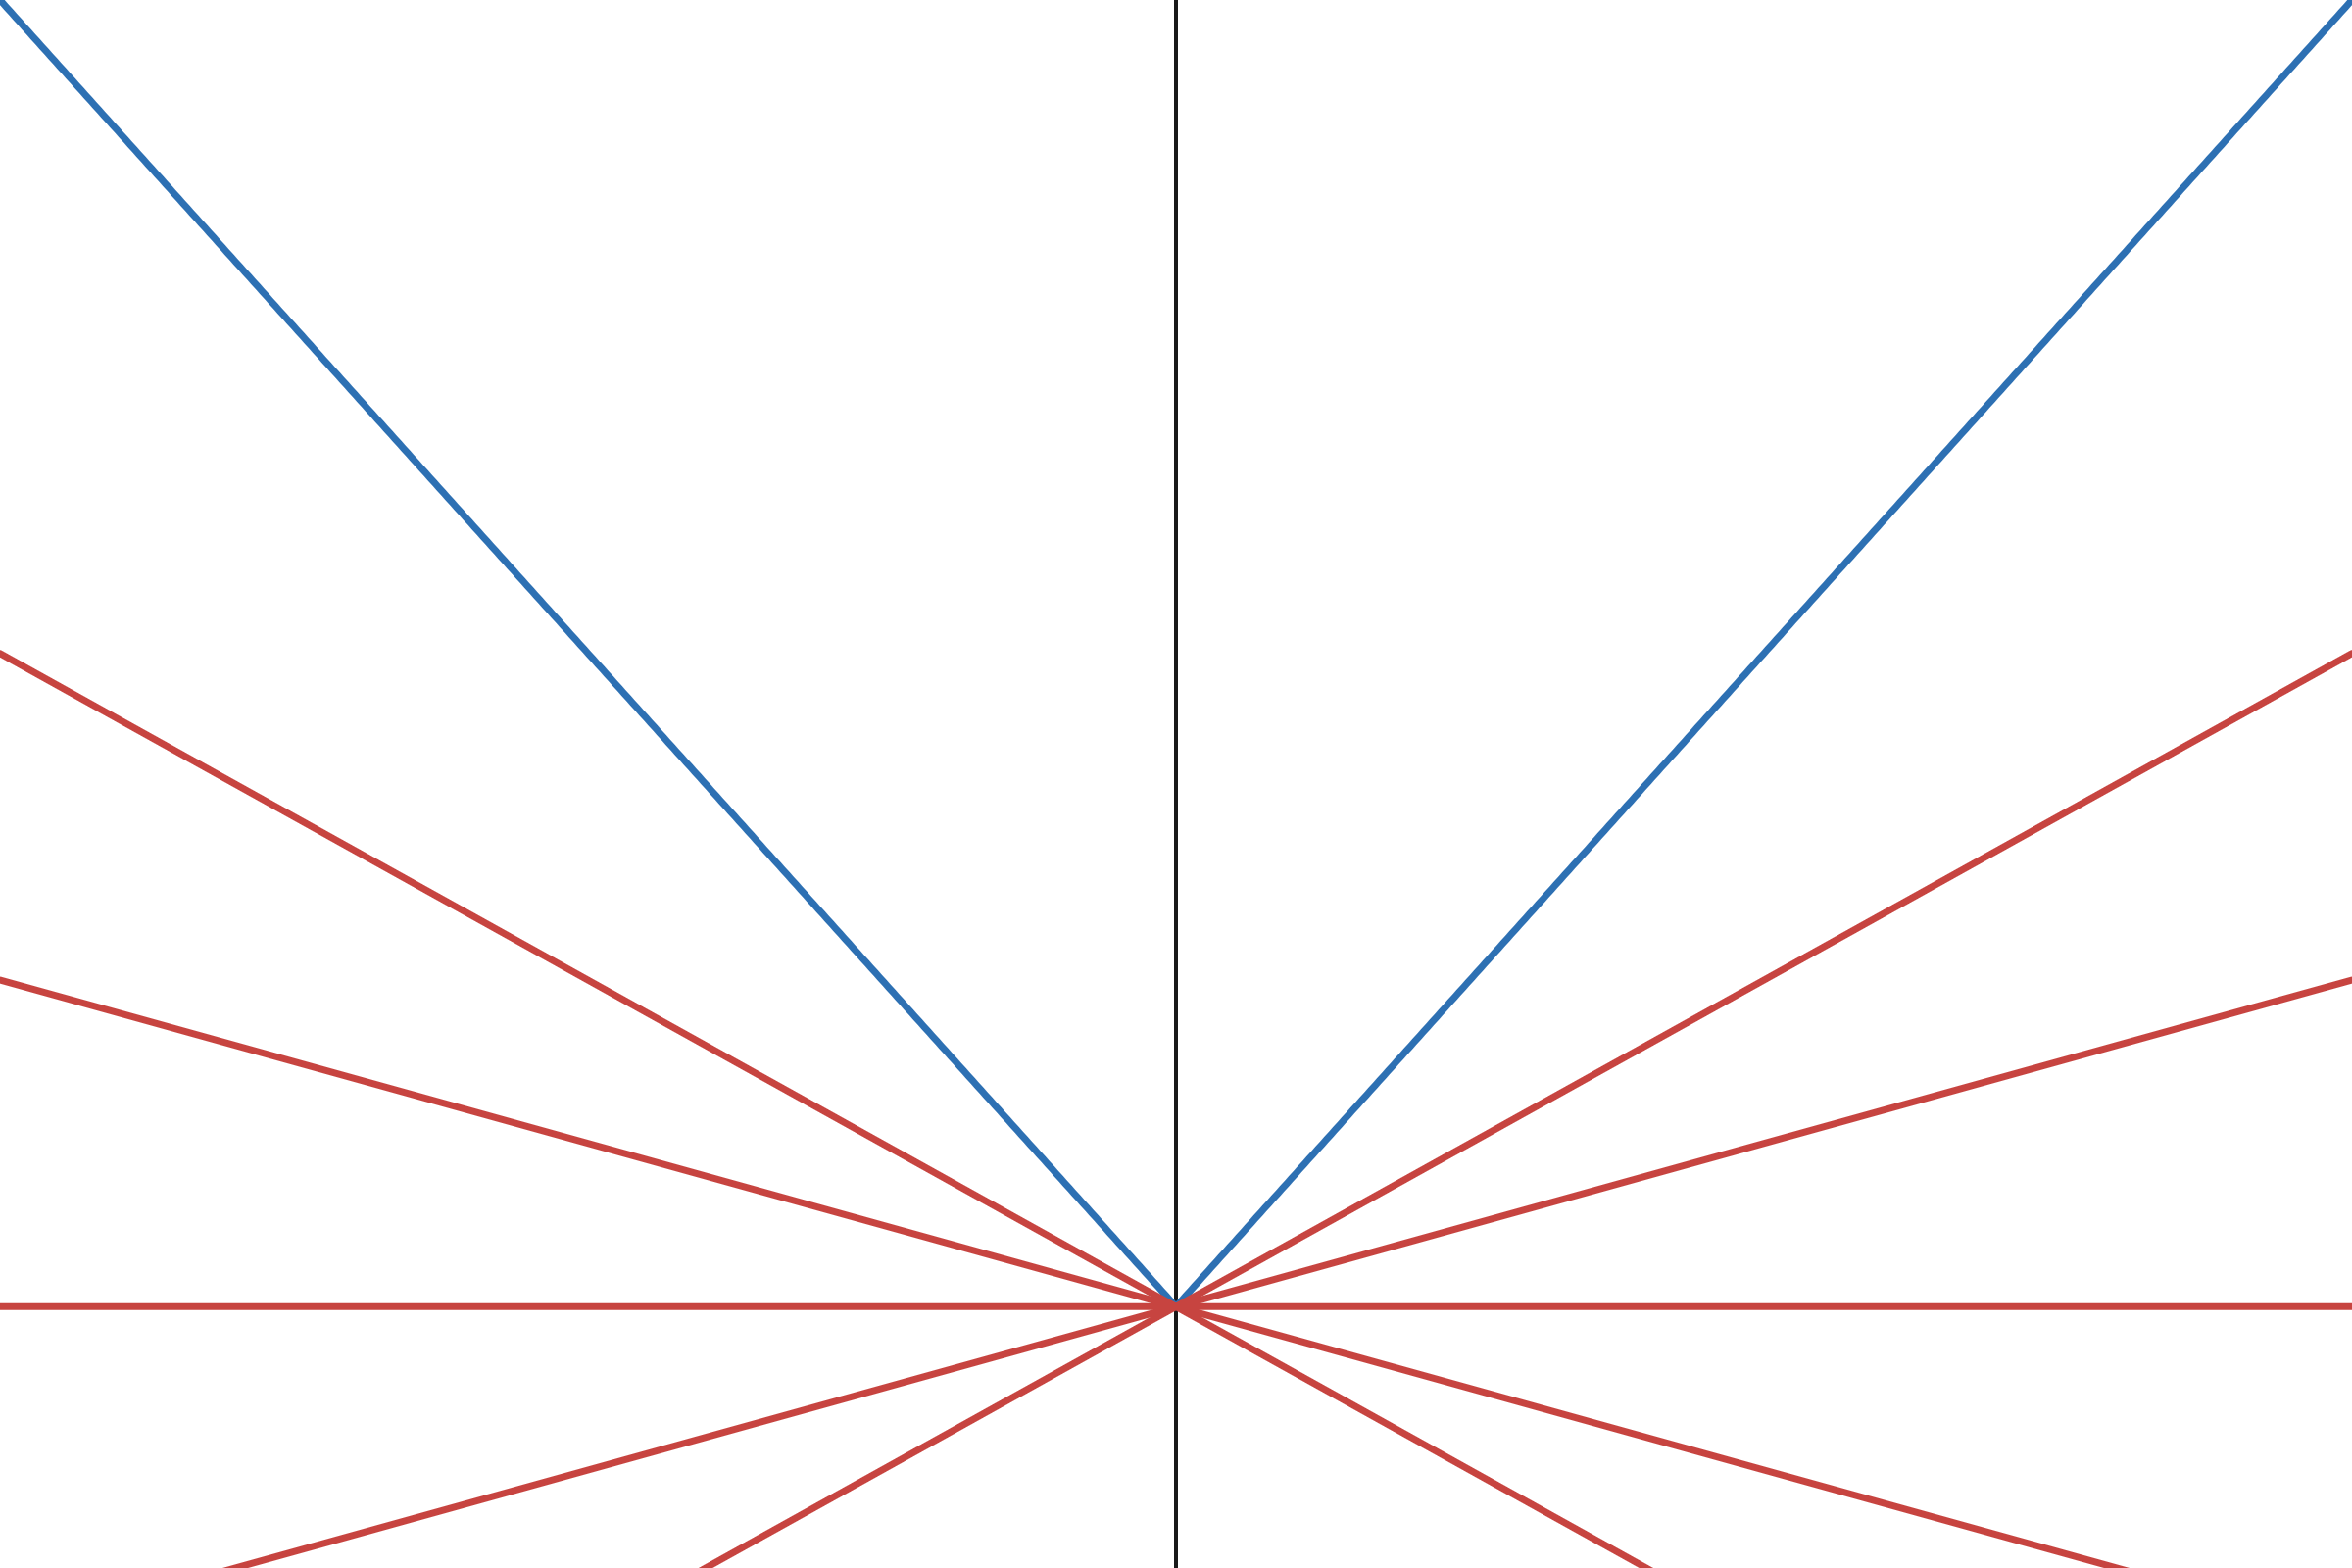
\includegraphics[width=0.5\linewidth]{Figures/abs_subgradients.png}
    \caption{Absolute value function (blue) with subgradients (red)}
    \label{fig:abs subgradients}
\end{figure}
In fact, we can say that any \(g \in [-1,1]\) would be a subgradient, and therefore \(\partial f(0) = [-1,1]\). But what about other points? For a point \(x > 0\), we can surmise that the only possible \(g = 1\), as any other value will leave some parts of our function beneath the resulting plane. Likewise for \(x < 0\), \(g = -1\). Using \eqref{eq:math subdifferential}, we can say
\begin{equation}\label{eq:abs subdifferential}
\partial f(x) = \begin{cases}
    \{-1\} & x < 0 \\
    [-1, 1] & x = 0\\
    \{1\} & x > 0
\end{cases}
\end{equation}
This can be compared against the derivative of \(f(x)\).
\begin{equation}\label{eq:abs derivative}
f'(x) = \begin{cases}
            -1 & x < 0\\
            1 & x > 0
\end{cases}
\end{equation}
We find that where the function is differentiable, the subdifferential contains only the gradient. There is only a difference where the function is not differentiable. Here we find that our set ranges between the two derivatives on either side of it. More formally, we can say that \(\partial f(x) = [a, b]\) such that
\begin{equation}\label{eq:subdifferential a def}
a = \lim_{y \rightarrow x^-} \frac{f(y)-f(x)}{y-x}
\end{equation}
\begin{equation}\label{eq:subdifferential b def}
b = \lim_{y \rightarrow x^+} \frac{f(y)-f(x)}{y-x}
\end{equation}
for one dimensional functions. We can note that for differentiable points \(a = b\), so this definition satisfies our observation up to this point.

\subsubsection{Properties}
There are a few important properties that we shall take note of. Proofs of these properties can be found in Appendix \ref{sec:subgradient properties proofs}.
\begin{itemize}
    \item If and only if the function is differentiable at \(x\), \(\partial f(x) = \{\nabla f(x)\}\)
    \item If and only if \(x^*\) is a global minimum, \(0 \in \partial f(x^*)\)
    \item \(\partial f(x)\) will always be a convex set
\end{itemize}

\subsection{Subgradient Methods}\label{sec:subgradient methods}
This section is predominantly adapted from \cite{boydparksubgradients} and \cite{boydxiaosubgradients}.

\subsubsection{Iteration Step}
Subgradient methods are a family of optimization techniques involving the same basic iteration step
\begin{equation}\label{eq:subgradient method iteration}
x^{(k+1)} = x^{(k)} - \alpha_k g^{(k)}
\end{equation}
where \(g^{(k)}\) is any subgradient at the point \(x^{(k)}\) and \(\alpha_k > 0\). There are a number of different methods of choosing \(\alpha_k\), which will be further explored in Section \ref{sec:choosing step size}. This formula can be seen to be very similar to gradient descent. In fact, can be observed that since the only subgradient at differentiable points is the gradient, all subgradient methods \textit{are} gradient descent in these sections, the only difference from regular gradient descent being our way of choosing step size. One notable difference from gradient descent is that subgradient methods are not descent methods; we are not guaranteed that every step will descend. For that reason we should have some method of tracking our best performing point.
\begin{equation}\label{eq:track best}
f^{(k)}_{best} = \min (f^{(k-1)}_{best}, f(x^{(k)}))
\end{equation}
And a corresponding \(i^{(k)}_{best}\) such that \(f(x^{(i^{(k)}_{best})}) = f^{(k)}_{best}\)
This would not be needed in a descent method, because our best performing point is always the last point.

\subsubsection{Convergence Proof}
We are focused on converging towards the optimum point within some error of margin. We begin by making the following assumptions
\begin{itemize}
    \item There exists a minimizer of \(f\) called \(x^*\), for which \(f^* = f(x^*)\)
    \item There exists some bounding value \(G\) for which \(\|g\|_2 \leq G, g \in \partial f(x), \forall x \in \dom f\)\footnote{One way that this assumption can be met is if the function satisfies the Lipschitz condition, but it is not the only way}\footnote{This assumption helps us greatly in our analysis, but it is not strictly necessary. There exist subgradient methods which can be proven to work even when this assumption does not hold \cite{boydparksubgradients}}
    \item There exists some known bounding value \(R\) such that \(R \geq \|x^{(1)}-x^*\|_2\)
\end{itemize}
Next we can write the following based on \eqref{eq:subgradient method iteration}
\begin{equation}
\|x^{(k+1)}-x^*\|^2_2 = \|x^{(k)} - \alpha_k g^{(k)}-x^*\|^2_2
\end{equation}
Focusing on the right side, we can multiply the quadratic out
\begin{equation}
\|x^{(k+1)}-x^*\|^2_2= \|x^{(k)}-x^*\|^2_2 - 2\alpha_k g^{(k)T}(x^{(k)}-x^*) + \alpha^2_k \|g^{(k)}\|^2_2
\end{equation}
Using the definition of subgradient from \eqref{eq:modified subradient def 2}, we can write
\begin{equation}
\|x^{(k+1)}-x^*\|^2_2 \leq \|x^{(k)}-x^*\|^2_2 - 2\alpha_k (f(x^{(k)})-f^*) + \alpha^2_k \|g^{(k)}\|^2_2
\end{equation}
Paying particular attention to the term \(\|x^{(k)}-x^*\|^2_2\), we can notice we have created a recursive inequality. If we perform a recursive substitution ultil reaching \(x^{(1)}\) we would find ourselves with the following inequality
\begin{equation}
\|x^{(k+1)}-x^*\|^2_2 \leq \|x^{(1)}-x^*\|^2_2 - 2\sum^k_{i=1}\alpha_i (f(x^{(i)})-f^*) + \sum^k_{i=1}\alpha^2_ki\|g^{(i)}\|^2_2
\end{equation}
We know that because of our bounding value \(R \geq \|x^{(1)}-x^*\|_2\) and because of the norm, \(\|x^{(k+1)}-x^*\|^2_2 \geq 0\), so we can write
\begin{equation}
    2\sum^k_{i=1}\alpha_i (f(x^{(i)})-f^*) \leq R^2  + \sum^k_{i=1}\alpha^2_ki\|g^{(i)}\|^2_2
\end{equation}
It follows readily from \eqref{eq:track best} that \(f^{(k)}_{best} \leq f(x^{(i)}) \forall 1 \leq i \leq k\), so we can say
\begin{equation}
    2\sum^k_{i=1}\alpha_i (f^{(k)}_{best}-f^*) \leq 2\sum^k_{i=1}\alpha_i (f(x^{(i)})-f^*) \leq R^2  + \sum^k_{i=1}\alpha^2_ki\|g^{(i)}\|^2_2
\end{equation}
And therefore
\begin{equation}
    f^{(k)}_{best}-f^* \leq \frac{R^2  + \sum^k_{i=1}\alpha^2_ki\|g^{(i)}\|^2_2}{2\sum^k_{i=1}\alpha_i}
\end{equation}
We can finish by applying our \(G\) bounding condition to \(\|g^{(k)}\|_2\), letting us write the final inequality
\begin{equation}
    f^{(k)}_{best}-f^* \leq \frac{R^2  + G^2 \sum^k_{i=1}\alpha^2_ki}{2\sum^k_{i=1}\alpha_i}
\end{equation}
Given that \(R\), \(G\), and \(\alpha_k\) are finite values, we can surmise that \(f^{(k)}_{best}\) approaches \(f^*\) within some small error bound that is dependent on \(\alpha_k\) and \(k\). It is evident from this that the means we use to choose \(\alpha_k\) will have significantly affect the error bound.

\subsection{Choosing Step Size}\label{sec:choosing step size}
There are many different methods of choosing the step size \(\alpha^{(k)}\). We will be discussing five broad categories in this section.

The first is a constant step size, where for some constant \(\alpha > 0\)
\begin{equation}\label{eq:constant step size}
\alpha^{(k)} = \alpha
\end{equation}

Second is a constant step length, where for some constant \(\gamma > 0\)
\begin{equation}\label{eq:constant step length}
\alpha^{(k)} = \frac{\gamma}{\|g^{(k)}\|_2}
\end{equation}
It can be easily proven that for this step size, \(\|x^{(k+1)}-x^{(k)}\|_2 = \gamma\)

\subsection{LASSO Regression}\label{sec:math lasso}

\section{Code Implementation}\label{sec:code}

\section{Numerical Results}\label{sec:results}

\section{Conclusion}\label{sec:conclusion}

\appendix
\subsection{Proving Subgradient Properties}\label{sec:subgradient properties proofs}
\subsubsection{When the Function is Differentiable}
We can begin by supposing that \(f\) is differentiable at \(x\), and therefore \(\nabla f(x)\) exists. Let us write a definition for each of its elements
\begin{equation}\label{eq:gradient elementwise def}
    \nabla f_i(x) = \lim_{y \rightarrow x} \frac{f(y)-f(x)}{y_i-x_i}
\end{equation}
And let us also rewrite \eqref{eq:modified subgradient def} with an elementwise sum
\begin{equation}\label{eq:subgradient elementwise sum}
f(x) - f(y)+ \sum^{n}_{i=1} g^T_i(y_i-x_i) \leq 0
\end{equation}
We can combine \eqref{eq:gradient elementwise def} and \eqref{eq:subgradient elementwise sum}
\begin{equation}
\lim_{y \rightarrow x} f(x) - f(y)+ \sum^{n}_{i=1} \nabla f_i(x)^T(y_i-x_i) \leq 0
\end{equation}
Substitute and simplify and we find that
\begin{equation}
\lim_{y \rightarrow x} f(x) - f(y)+ \sum^{n}_{i=1} \nabla f_i(x)^T(y_i-x_i) = 0
\end{equation}
If we are interested in trying an alternate \(g \neq \nabla f_i(x)\), we can say that a particular \(g_i\) would be invalid if
\begin{equation}\label{eq:differentiable cookie}
g_i(y_i-x_i) > \nabla f_i(x)(y_i-x_i)
\end{equation}
If \(g_i > \nabla f_i(x)\) and \(y_i > x_i\), this condition is fulfilled and therefore no values of \(g_i > \nabla f_i(x)\) are valid. Likewise, if \(g_i < \nabla f_i(x)\) and \(y_i < x_i\) this condition is fulfilled and therefore no values of \(g_i < \nabla f_i(x)\) are valid. Therefore the only valid values for every \(g_i = \nabla f_i(x)\), so the only valid \(g = \nabla f(x)\) if \(\nabla f(x)\) exists.

\subsubsection{Global Minimum}
If \(x^*\) is a global minimum it must be true that \(\forall y \in \dom f\)
\begin{equation}\label{eq:global min def}
f(x^*) \leq f(y)
\end{equation}
If we have \(g\) equal to the zero vector in \eqref{eq:subgradient def}, we end up removing the second term, so we end up with
\begin{equation}\label{eq:zero vector subgradient}
f(y) \geq f(x)
\end{equation}
We can trivially redefine \(x = x^*\) to derive \eqref{eq:global min def}. Therefore \(x^*\) is optimal if and only if the zero vecctor is included in its subdifferential.

\subsubsection{Convexity}
We can view \eqref{eq:modified subgradient def} as defining a halfspace in terms of \(x, y, f\). From \eqref{eq:math subdifferential} we can see that \(\partial f(x)\) is composed of intersections of these halfspaces. Since halfspaces are always convex and the intersection of convex sets is always convex, \(\partial f(x)\) must be a convex set.

\bibliographystyle{IEEEtran}
\bibliography{refs}

\end{document}